\BigLetter{D}{efining}, designing and orchestrating a distributed system used as a file archive is a compromising process of electing architecture, communication and security, etc. This chapter describes and discusses the choices and opportunities regarding what henceforward will be denoted as \CodeNameFull. 

\begin{figure}
	\centering
	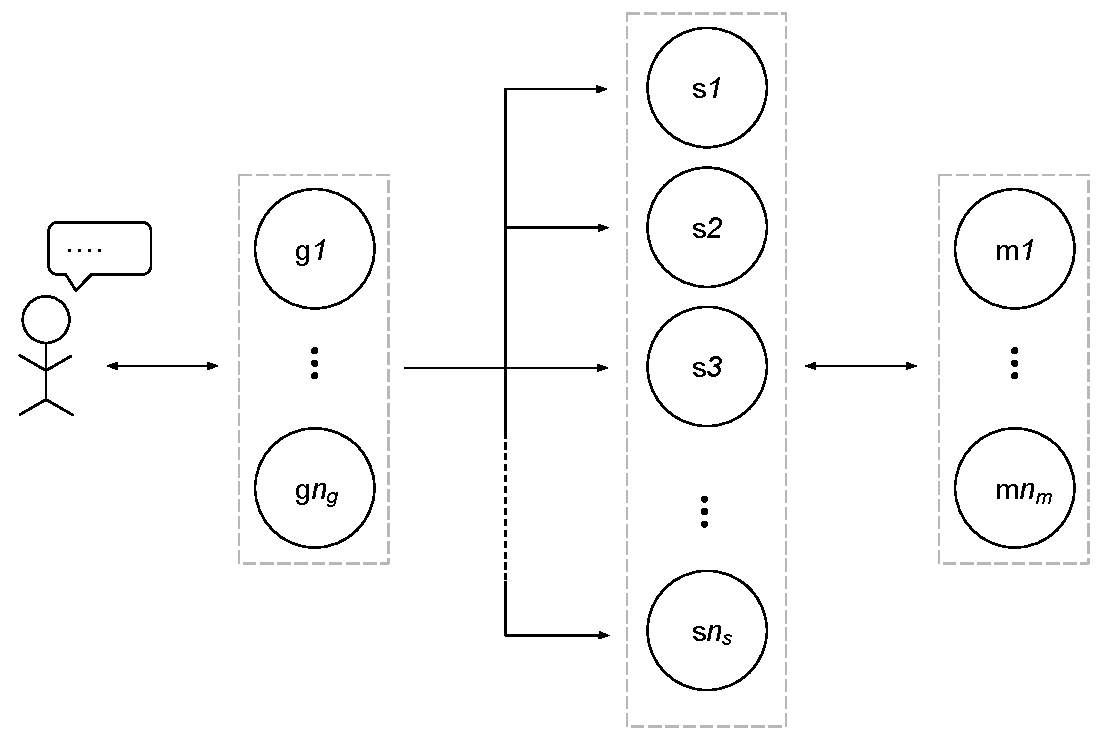
\includegraphics[scale=0.60]{pdf/sofa-overview.pdf}
	\caption[General overview of \CodeName]{General overview of \CodeName and the participating components and their associates, including $n_g$ gateways denoted by $\text{g}1 \ldots \text{g}n_g$, $n_s$ storage nodes by $\text{s}1 \ldots \text{s}n_s$ and $n_m$ monitors by $\text{m}1 \ldots \text{m}n_m$. \label{fig:sofa-overview}}
\end{figure}

\section{Overview}
This project, as mentioned is an alternative to the existing file archives targeting big data analysis frameworks; the architectural structure will be influenced and inspired by those described in the related work section (\ref{sec:related}) among others, both by characteristics and feature, but certainly from inaccuracies too. 
\newline

The architecture of file archive seeks to model an interpretation of a Storage Area Network (SAN) primarily used for research and scientific related big data analysis operating in a trusted homogeneous computing environment. The illustration at Figure \ref{fig:sofa-overview} depicts the general overview and flow of the system just described, where each component are examined subsequently in chapter \ref{chp:components}.

\section{Hardware} \label{sec:hardware}
The framework will first and foremost be designed to execute on a homogeneous collection of machines connected to a network, \ie a cluster, the choice could have been a grid (a collection of heterogeneous machines) too. 

The fact that the underlying component is a file archive related system built by bricks (outlined in definition \ref{def:brick}) make clusters an obvious choice for a prototype.

\vspace*{3mm}
\begin{definition}[Brick] \label{def:brick}
\textit{A brick is defined as a component of a homogeneous distributed system, where each of them is functional equivalent and are contributing uniformly and have equal rights.}
\end{definition}
\vspace*{3mm}

The implementation will be targeted inexpensive commodity hardware just as \eg Dynamo or the Google File System (both described as part of section \ref{sec:related}) and will be assembled by JBODs (described in defintion \ref{def:jbod}) for this first version.

\vspace*{3mm}
\begin{definition}[JBOD] \label{def:jbod}
\textit{It is an acronym for Just a Bunch of Disks and is a hardware architecture with multiple hard drives, but without configuration of RAID and thus doesn't provide redundancy nor performance improvements.}
\end{definition}


\section{Architectural style}
Section \ref{sec:architectures} describes a collection of different distributed system architectures\cite{Tanenbaum:2006:DSP:1202502}, where the architecture of the project will be affected by knowledge and benefits from existing solutions (described in section \ref{sec:related}). 
\newline

The result will seek to model the notion of a hybrid related distributed system with a decentralized collection of interconnected storage nodes accessible by potentially multiple replicated stateless gateway servers and observed by one or more monitors.

\begin{figure}[h!]
	\centering
	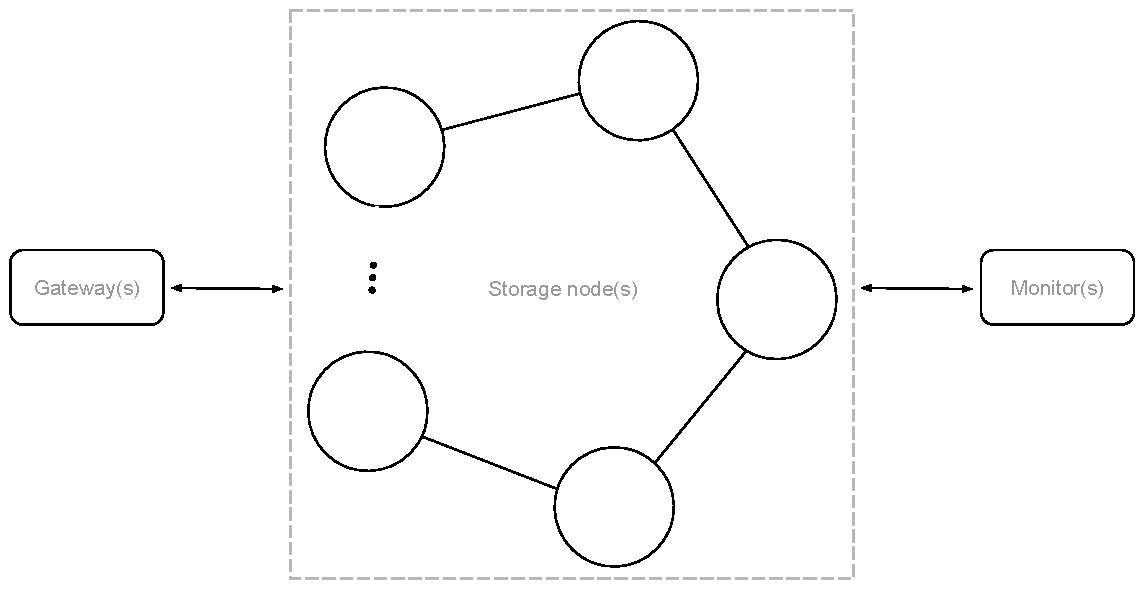
\includegraphics[scale=0.7]{pdf/architecture-overview.pdf}
	\caption[Architectural overview]{Architectural overview of the hybrid related distributed system reflecting a zero-hop distributed hash table ring of storage nodes. \label{fig:architecture-overview}}
\end{figure}

The architecture of the interconnected storage nodes (depicted at Figure \ref{fig:architecture-overview}) is highly influenced by Dynamo and will reflect a zero-hop distributed hash table (DHT, described as part of the decentralized architecture in section \ref{sec:architectures}) and thus provides full data consistency concerning the CAP theorem, \reference{def:cap}{sec:cap}. Unfortunately, this also means that complexity regarding the consistency protocol increases at a membership level.
\newline

The design and structure of the storage node will be described as part of chapter \ref{chp:nodes} in section \ref{sec:storage}, the gateway in section \ref{sec:gateway} and the monitor in chapter \ref{sec:monitor}.

\section{Communication}


\section{Partitioning and distribution} \label{sec:pandd}
The partitioning and distribution protocol in \CodeName is based on consistent hashing (\reference{def:ch}{sec:partitioning}) and the round-robin load balancing algorithm (described in definition \ref{def:rr}). The downside of this distribution algorithm is that it does not take state, availability and workload among other properties of the servers into account. However, one of the presumptions (described in section \ref{sec:presumptions}) is that the framework primarily is expected to be operating in homogeneous and high-performance computing environment like a cluster.
\vspace*{3mm}

\begin{definition}[Round-robin] \label{def:rr}
\textit{A simple, fair share and starvation free load balancing algorithm that is easy to implement. The algorithm is distributing elements until there are no more among the available servers in a one-by-one or chunk-by-chunk fashion, thus the name of the algorithm.}
\end{definition}
\vspace*{3mm}

\begin{figure}[h!]
	\centering
	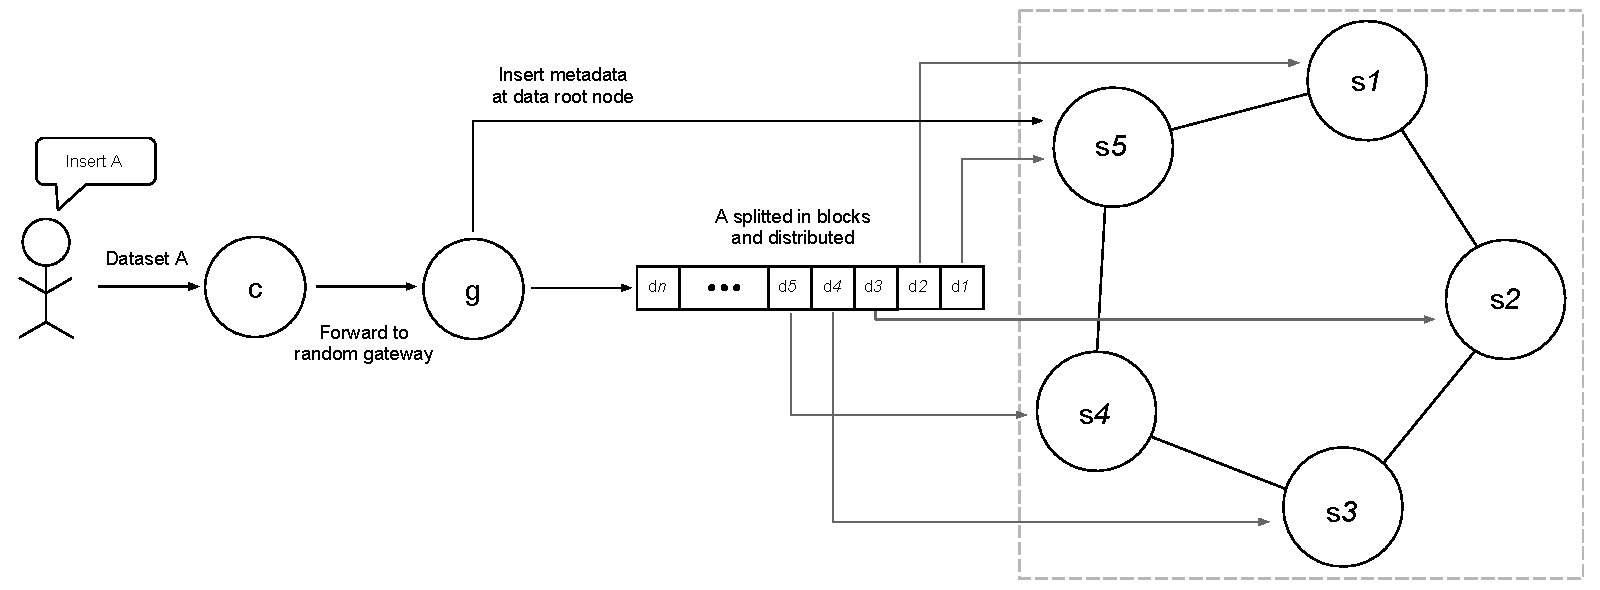
\includegraphics[scale=0.5]{pdf/rr-partitioning.pdf}
	\caption[Overview of the partitioning and data distribution protocol]{General flow of the partitioning and data distribution protocol in \CodeName, assuming one gateway server \textit{g} and a client \textit{c} attempting to insert data \textit{A} consisting of \textit{n} blocks $\text{d}1 \ldots \text{d}n$.\label{fig:rr-partitioning}}
\end{figure}

\vspace*{3mm}
Figure \ref{fig:rr-partitioning} illustrates the general flow of the preferred partitioning and distribution protocol. The data is distributed from the client to an arbitrary gateway server, where it is assigned a unique identifier using consistent hashing (as in Amazons Dynamo project) and partitioned into approximately\footnote{As described in section \ref{sec:objectives} is one of the ambitions to store arbitrary sized block.} equal block sizes. The blocks are distributed in a round-robin fashion to the storage nodes, after the metadata for the data is assigned to the root server\footnote{The server responsible for the data, which is determined by the identifier.}. It is presumably sufficient as a distribution protocol under the assumptions outlined in section \ref{sec:assumption} with regards to big data.

\section{Naming and virtualization} \label{sec:virtualization}
A requirement is that each instance of \CodeNameFull associated with a specific global instance name (described in section \ref{sec:configuration}) \eg based on the research area or even specific data types. This name is predominantly used to virtualize components, data, and caches and thereby supporting multiple executions of \CodeName instances at once with own domain.
\newline

Elements in the framework are identified using a predominantly structured naming based technique (described in \cite{Tanenbaum:2006:DSP:1202502}), where each semicolon denotes an explicit and more specific context. 

\subsubsection*{Nodes}
The pattern of the naming scheme of node components (depicted at as a general overview at Figure \ref{fig:sofa-overview} and described in chapter \ref{chp:components}) are characterized as following:
\vspace*{2mm}
\begin{equation*}
	\texttt{sofa}:<\text{instance name}>:<\text{type ref}>:<\text{sequence number}>
\end{equation*}
, where \texttt{type ref} is one of following component types: gateway, storage or monitor and \texttt{sequence number} is a positive increasing number in range $0\ldots n$ where $n$ is either the number of gateways, storage nodes or monitors respectively

\subsubsection*{Data}
\begin{equation*}
	<\text{instance name}>:<\text{data type}>:<\text{data name}>
\end{equation*}
\vspace*{1mm}

The naming scheme of data which also are described in chapter \ref{chp:components} are defined as above, where \texttt{instance name} is the same as above, the \texttt{data type} is an optional parameter if the framework supports multiple types. The name of the data is required to be unique and specified as \texttt{data name}. The \texttt{sofa} identifier is not necessary since the data is only accessible in a sofa based context.
\newline

As mentioned in the preceding sections \textit{architectural style} and \textit{partitioning and distribution} are slaves organized in a zero-hop distributed hash table based architecture with a user-specific limited key-space size (system configurations are described in details in section \ref{sec:configuration}). The full name is hashed\footnote{\texttt{hash(}data-name\texttt{)} \texttt{mod} \texttt{size(}key-space\texttt{)}} to generate an anonymous unique identifier to insert new data and localize existing data.

\section{Redundancy and replication}
Redundancy in \CodeName is carried out using \eg software RAID-Z in ZFS (described in Description \ref{def:zfs}), which provides block-level striping with double distributed parity, that ensures fault tolerance by upto two failed drives. The motivation for this is that the existing replication protocols in \eg Hadoop, and the Google File System described in section \ref{sec:related} and \ref{sec:replication} are using a vast amount of space and communication are too expensive considering that the primary usage of this is big datasets.
\newline

If redundancy protocol however is based on erasure codes then it is no longer replication, but fault tolerance with a degree of durability. This type of responsibility is in this system carried out in hardware by the JBODs, such that there is no need for the extensive amount of network data transfer.
\vspace*{2mm}

\begin{definition}[ZFS] \label{def:zfs}
\textit{It is composed of one or more virtual storage pools which are a collection of virtual devices that can be interpreted as a RAID (Redundant Array of Independent Disks) set in a standard file system.}
\newline

\textit{ZFS is an extensive 128-bit addressable file system that always is consistent on disk, this is because it performs a copy on write operation when adding new data, \ie writing modified data into a new space and reuse the old space in the future, thus eliminating the write hole error (corrupted file system) \eg on power loss.}
\end{definition}
\vspace*{2mm}

\section{Recovery} \label{sec:recovery}
The RAID-Z configuration described in the previous section with the purpose of \eg replication are also used as a basic recovery protocol to conceal disk failures. A second recovery initiative is redundant multipaths to efficiently hide server error - a technique that will be described forthwith.
\newline

The system will run on economical low-cost hardware such as JBODs (outlined in definition \ref{def:jbod}) as explained in section \ref{sec:hardware}. Having SAS-controlled\footnote{Serial Attached SCSI: serial point-to-point protocol for moving data} disks enables fail-over features such as multipathing (definition \ref{def:multipath}) that allows redundant data paths between host servers and the block-level devices. Figure \ref{fig:1host-1disk} illustrates a simple example with one host and one array of disks, where:

\begin{itemize}
	\item \textbf{HBA} (Host Bus Adapter) is the local controller on the computer that connects it to other storage or network devices.
	\item \textbf{SIM} (SAS Interface Module) is the storage device controller.
\end{itemize}
\vspace*{3mm}

Figure \ref{fig:2host-2disk} includes another more complex example to show the scalability with multiple hosts and disks.

\begin{figure}[h!]
	\centering
	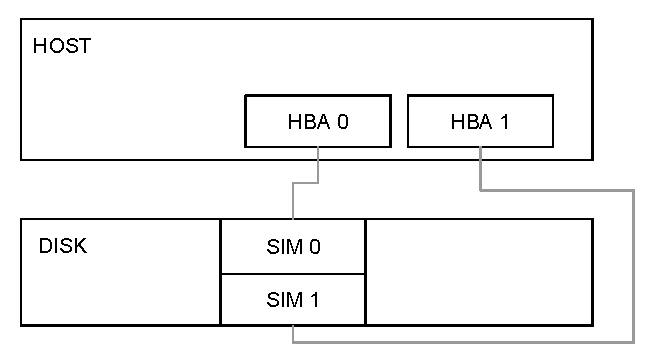
\includegraphics[scale=0.75]{pdf/1host-1disk.pdf}
	\caption[Simple JBod setup]{JBod setup with one host and one array of disks.\label{fig:1host-1disk}}
\end{figure}

\begin{definition}[DM Multipath] \label{def:multipath}
\textit{Multipathing is a Linux operating system device mapper for SAS-controlled hard drives that provides I/O fail-over and load balancing, by having numerous paths between host and disk. The configuration of DM Multipath is handled at an operating system level and the device controllers on the storage disks is unaware of such configurations.}
\end{definition}

\begin{figure}[h!]
	\centering
	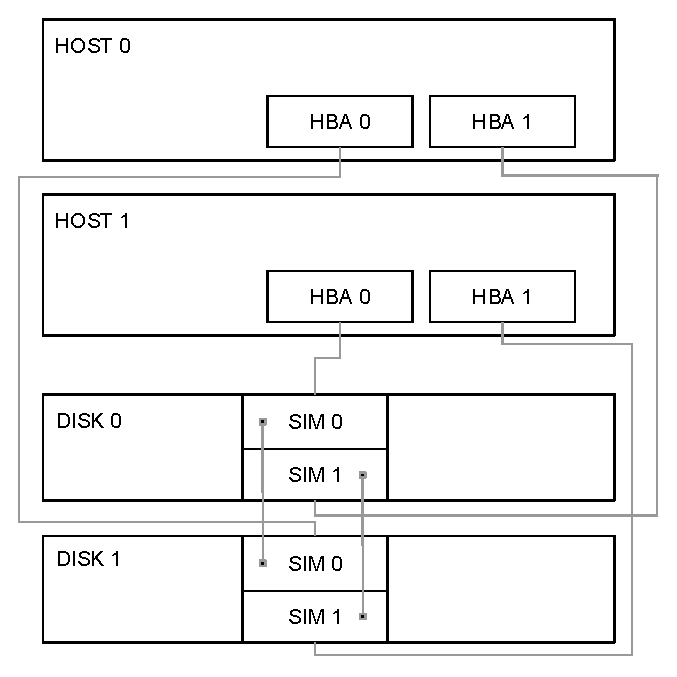
\includegraphics[scale=0.75]{pdf/2host-2disk.pdf}
	\caption[Complex JBod setup]{JBod setup with multiple hosts and multiple disks. \label{fig:2host-2disk}}
\end{figure}

\section{Security} \label{sec:security}
The focus on data integrity and security have predominantly been given low priority, since the system is expected to execute in a trusted environment, exactly like Amazon Dynamo, thus it is intentionally implemented without internal authentication or authorization.
\newline

Nevertheless, security is evidently an influential component and property at the boundary of the system, one of many actions is \eg using the secure HTTPS connection on the network requests to the entry gateway servers instead of ordinary HTTP. Validation of user input is most certainly also a reasonable action when it comes to security.
